\section{Analysis and Graphics}

The analysis of the first dataset is more comprehensive, with tables and illustrative graphs for different 
numbers of documents. In contrast, the analysis of the second dataset is more limited due to constraints that 
will be discussed shortly, which hindered the generation of results for all scenarios.
\subsection{Analysis for First dataset}

 \subsubsection{Insertion Performance}

 Table \ref{tab:insercao_completa} presents performance metrics for insertion operations,
 for different quantities of documents ($n$), where \textbf{Time (s)} measures the total duration of the process, \textbf{Comparisons} counts the total number
 of comparison operations between nodes, and \textbf{Relative Efficiency} indicates the comparative gain
 in relation to the BST.

 \begin{table}[H]
     \centering
     \begin{tabular}{|c|c|c|c|c|c|}
     \hline
     \textbf{n (docs)} & \textbf{Words} & \textbf{Structure} & \textbf{Time (s)} & \textbf{Comparisons} & \textbf{Relative Efficiency} \\
     \hline
     \multirow{3}{*}{10} & \multirow{3}{*}{1.279} & BST & 0.021 & 38,668 & 1.00 \\
     & & AVL & 0.020 & 39,187 & 0.99 \\
     & & RBT & 0.021 & 34,948 & 1.11 \\
     \hline
     \multirow{3}{*}{100} & \multirow{3}{*}{6.634} & BST & 0.230 & 548,119 & 1.00 \\
     & & AVL & 0.233 & 507,573 & 1.08 \\
     & & RBT & 0.229 & 484,434 & 1.13 \\
     \hline
     \multirow{3}{*}{1000} & \multirow{3}{*}{16.985} & BST & 1.965 & 5,689,724 & 1.00 \\
     & & AVL & 1.912 & 5,037,297 & 1.13 \\
     & & RBT & 1.922 & 5,028,881 & 1.13 \\
     \hline
     \multirow{3}{*}{5000} & \multirow{3}{*}{20.190} & BST & 10.763 & 29,821,186 & 1.00 \\
     & & AVL & 10.556 & 26,207,636 & 1.14 \\
     & & RBT & 10.503 & 26,660,495 & 1.12 \\
     \hline
     \multirow{3}{*}{10103} & \multirow{3}{*}{20.273} & BST & 24.268 & 59,612,852 & 1.00 \\
     & & AVL & 23.721 & 52,301,192 & 1.14 \\
     & & RBT & 23.678 & 53,405,044 & 1.12 \\
     \hline
     \end{tabular}
     \caption{Insertion performance with relative efficiency compared to BST}
     \label{tab:insercao_completa}
 \end{table}

 Despite the additional balancing operations, AVL and RBT show comparable
 or superior efficiency to BST in insertions. For large volumes ($n \geq 1000$), both perform 12-14\% fewer
 comparisons, which is reflected in consistently lower times. The RBT stands out in smaller scenarios
 ($n = 10$) with an 11\% gain in relative efficiency, while the AVL maintains a stable advantage
 (14\%) in larger sets ($n \geq 5000$).

 Figure \ref{fig:timedist} demonstrates the distribution of insertion time,
 showing that RBT has the lowest temporal variability among the analyzed structures,
 while BST exhibits the greatest dispersion in insertion times.

 \begin{figure}[H]
     \centering
     \includegraphics[width=0.8\linewidth]{img/Graph_5_10103.pdf}
     \caption{Number of comparisons by number of words}
     \label{fig:timedist}
 \end{figure}

 Figure \ref{fig:cumulativedist} reveals that, although insertions in AVL and RBT
 involve additional balancing operations, the superior efficiency in search operations
 compensates for this initial cost, particularly in datasets with many repeated words.

 \begin{figure}[H]
     \centering
     \includegraphics[width=0.8\linewidth]{img/Graph_4_10103.pdf}
     \caption{Number of comparisons by number of words}
     \label{fig:cumulativedist}
 \end{figure}
Figure \ref{fig:mean-log} shows the average number of comparisons for every 100 new words inserted into the trees, indicating that the insertion complexity in each tree is proportional to $log_2(n)$. It can be observed that the differences between the trees become noticeable only after a significant number of words have been inserted—when balancing begins to affect the number of comparisons more evidently.

The RBT exhibits the lowest insertion complexity, which is due to its balancing mechanism being similar to the AVL's, but requiring fewer comparisons to maintain balance. The BST lies between AVL and RBT: although it performs no additional comparisons for balancing, finding the parent of the new node typically requires more comparisons than in RBT, making its insertion less efficient overall.

Despite being the most balanced tree, the AVL has the highest average number of comparisons. This is because, even though its search is the most efficient, the need to update the heights of ancestor nodes after each insertion significantly increases its average, making it nearly twice as high as the average number of comparisons required for search operations.

\begin{figure}[H]
     \centering
     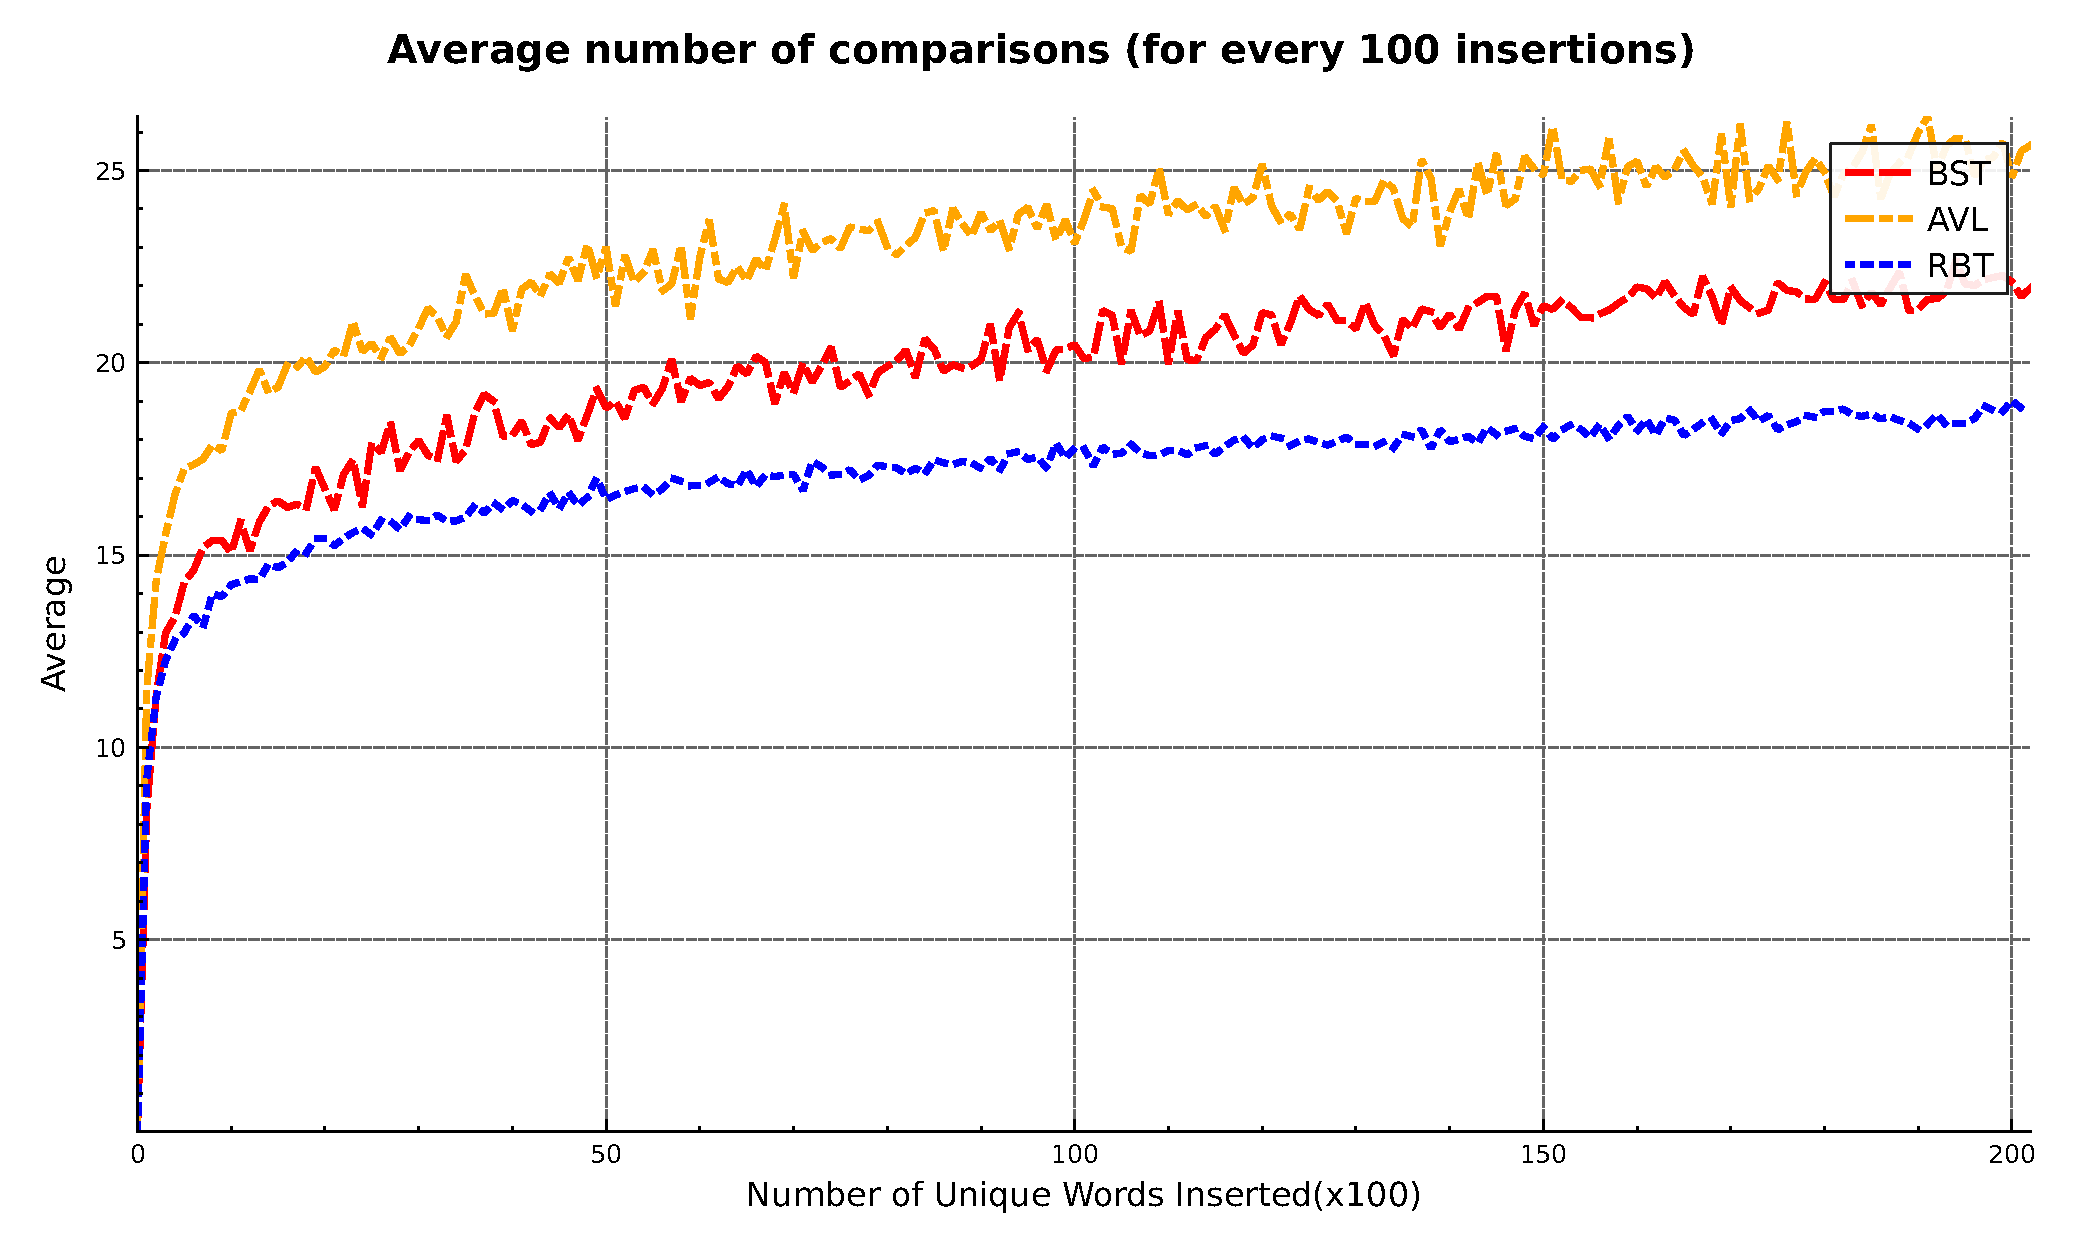
\includegraphics[width=0.8\linewidth]{img/Graph_3_20273.pdf}
     \caption{Number of comparisons by number of words}
     \label{fig:mean-log}
\end{figure}


 \subsubsection{Search Performance}

 Table \ref{tab:busca_completa} displays results for search operations for different numbers
 of documents ($n$), with \textbf{Time (ms)}
 representing the average duration per operation, \textbf{Comparisons} showing the average number of comparisons per search,
 and \textbf{Relative Efficiency} indicates the gain in the number of comparisons relative to the BST.

 \begin{table}[H]
     \centering
     \begin{tabular}{|c|c|c|c|c|c|}
     \hline
     \textbf{n (docs)} & \textbf{Words} & \textbf{Structure} & \textbf{Time (ms)} & \textbf{Comparisons} & \textbf{Relative Efficiency} \\
     \hline
     \multirow{3}{*}{10} & \multirow{3}{*}{1.279} & BST & 2.477 & 16,657 & 1.00 \\
     & & AVL & 2.466 & 12,252 & 1.264 \\
     & & RBT & 2.422 & 12,312 & 1.261 \\
     \hline
     \multirow{3}{*}{100} & \multirow{3}{*}{6.634} & BST & 12.755 & 108,933 & 1.00 \\
     & & AVL & 12.215 & 79,420 & 1.271 \\
     & & RBT & 12.321 & 79,940 & 1.266 \\
     \hline
     \multirow{3}{*}{1000} & \multirow{3}{*}{16.985} & BST & 28.333 & 313,739 & 1.00 \\
     & & AVL & 26.595 & 226,639 & 1.278 \\
     & & RBT & 27.285 & 228,744 & 1.271 \\
     \hline
     \multirow{3}{*}{5000} & \multirow{3}{*}{20.190} & BST & 34.393 & 380,500 & 1.00 \\
     & & AVL & 33.366 & 274,630 & 1.278 \\
     & & RBT & 34.111 & 277,234 & 1.271 \\
     \hline
     \multirow{3}{*}{10103} & \multirow{3}{*}{20.273} & BST & 35.627 & 382,313 & 1.00 \\
     & & AVL & 34.379 & 275,883 & 1.278 \\
     & & RBT & 34.022 & 278,510 & 1.271 \\
     \hline
     \end{tabular}
     \caption{Search performance with relative efficiency compared to BST}
     \label{tab:busca_completa}
 \end{table}


 The balanced trees demonstrate expressive gains in search operations, consistently reducing
 comparisons by 26-28\% relative to the BST across all scales. This optimization is directly reflected in the time:
 the AVL and RBT maintain a temporal advantage in all cases. It is important to note that the analysis of search time for small
 $n$ is imprecise; however, for large $n$, the analysis closely approximates the analysis of the number of comparisons.
analys
 Figure \ref{fig:comparacoes} presents the distribution of the number of comparisons made
 during searches, as a function of the number of words, for the three analyzed structures:
 BST, AVL, and RBT. It is observed that the balanced trees (AVL and RBT) have distributions
 that are significantly more concentrated around a single value, with frequency peaks at
 approximately 14 comparisons—indicating that most words are located after this
 number of steps. In the BST, the distribution is more dispersed, with a peak
 shifted to around 19 comparisons, reflecting greater variability compared to the balanced trees.

 \begin{figure}[H]
     \centering
     \includegraphics[width=0.8\linewidth]{img/Graph_6_10103.pdf}
     \caption{Number of comparisons by number of words}
     \label{fig:comparacoes}
 \end{figure}


 In particular, this is the level of the tree that has the most nodes. This implies that searches in AVL and RBT are not only faster but also more predictable.
 On the other hand, the BST—by not guaranteeing balancing—can suffer structural degradations in unfavorable scenarios, which leads to an increase in the average number of comparisons.

 \subsubsection{Maximum and Minimum Branch}

 Table \ref{tab:altura_completa} shows the tree height statistics,
 where \textbf{Max. Dist} represents the longest distance from the root to any leaf,
 \textbf{Min. Dist} indicates the shortest distance from the root to a leaf, \textbf{Difference}
 calculates the variation between these heights, and \textbf{Ratio} expresses the proportion between maximum
 and minimum height, with values close to 1 being indicative of better balancing.

 \begin{table}[H]
     \centering
     \begin{tabular}{|c|c|c|c|c|c|c|}
     \hline
     \textbf{n (docs)} & \textbf{Words} & \textbf{Structure} & \textbf{Max. Dist} & \textbf{Min. Dist} & \textbf{Difference} & \textbf{Ratio} \\
     \hline
     \multirow{3}{*}{10} & \multirow{3}{*}{1.279} & BST & 23 & 4 & 19 & 5.75 \\
     & & AVL & 11 & 7 & 4 & 1.57 \\
     & & RBT & 12 & 7 & 5 & 1.71 \\
     \hline
     \multirow{3}{*}{100} & \multirow{3}{*}{6.634} & BST & 29 & 5 & 24 & 5.80 \\
     & & AVL & 14 & 9 & 5 & 1.56 \\
     & & RBT & 15 & 9 & 6 & 1.67 \\
     \hline
     \multirow{3}{*}{1000} & \multirow{3}{*}{16.985} & BST & 34 & 5 & 29 & 6.80 \\
     & & AVL & 16 & 10 & 6 & 1.60 \\
     & & RBT & 16 & 10 & 6 & 1.60 \\
     \hline
     \multirow{3}{*}{5000} & \multirow{3}{*}{20.190} & BST & 36 & 5 & 31 & 7.20 \\
     & & AVL & 16 & 10 & 6 & 1.60 \\
     & & RBT & 17 & 10 & 7 & 1.70 \\
     \hline
     \multirow{3}{*}{10103} & \multirow{3}{*}{20.273} & BST & 36 & 5 & 31 & 7.20 \\
     & & AVL & 16 & 10 & 6 & 1.60 \\
     & & RBT & 17 & 10 & 7 & 1.70 \\
     \hline
     \end{tabular}
     \caption{Tree height statistics for different data volumes}
     \label{tab:altura_completa}
 \end{table}

 It is noted that even for small sets ($n = 10$), the BST already exhibits a significant
 disparity between minimum and maximum heights (ratio of 5.75). As the data volume
 increases, this difference widens, reaching ratios greater than 7. In contrast, the balanced
 structures (AVL and RBT) maintain height differences of less than 7 nodes and maximum ratios of 1.70,
 demonstrating consistently stable behavior regardless of the data scale. The following graphs
 are on a logarithmic scale for better visualization.

 \begin{figure}[H]
     \centering
     \includegraphics[width=0.75\linewidth]{img/Graph_1_10103.pdf}
     \caption{Tree height per insertion}
     \label{fig:maiorgalho}
 \end{figure}

 \begin{figure}[H]
     \centering
     \includegraphics[width=0.75\linewidth]{img/Graph_2_10103.pdf}
     \caption{Tree height per insertion}
     \label{fig:menorgalho}
 \end{figure}

 Note that, in general, as evidenced by figures \ref{fig:maiorgalho}-\ref{fig:menorgalho}, in AVL and RBT trees—being balanced—it is necessary to insert a larger quantity
 of nodes for the total height of the tree (or the size of the smallest branch) to increase. Their balancing restricts the excessive growth of the branches.
 On the other hand, in the BST, this behavior is not guaranteed: in pathological cases, such as ordered insertions,
 two new nodes may be sufficient to increase the tree height by two units.

 Note that in figure \ref{fig:menorgalho}, there was a moment when the size of the smallest branch decreased. At first,
 we might think this is incorrect. But in fact, this is not a problem,
 as it can really occur, see the example:

 In figure \ref{fig:bef645} we have an AVL tree such that the size of the smallest branch is 4, and in figure
 \ref{fig:af645} it is the same tree after inserting node $645$. After this insertion,
 this node becomes the root and the size of the smallest branch will be 3.

 \begin{figure}[H]
     \centering
     \begin{minipage}{0.46\linewidth}
         \centering
         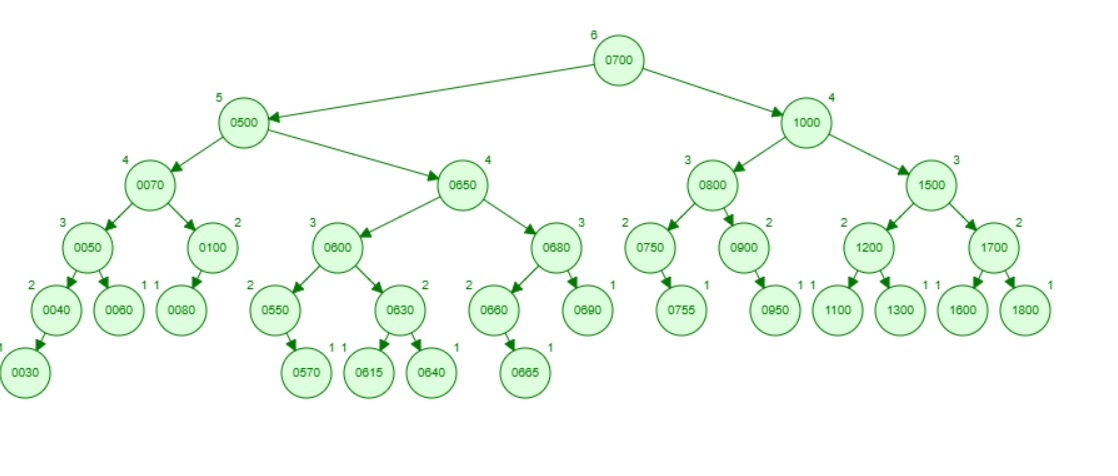
\includegraphics[width=\linewidth]{img/avl_before.jpeg}
         \caption{Before inserting node 645}
         \label{fig:bef645}
     \end{minipage}
     \hfill
     \begin{minipage}{0.48\linewidth}
         \centering
         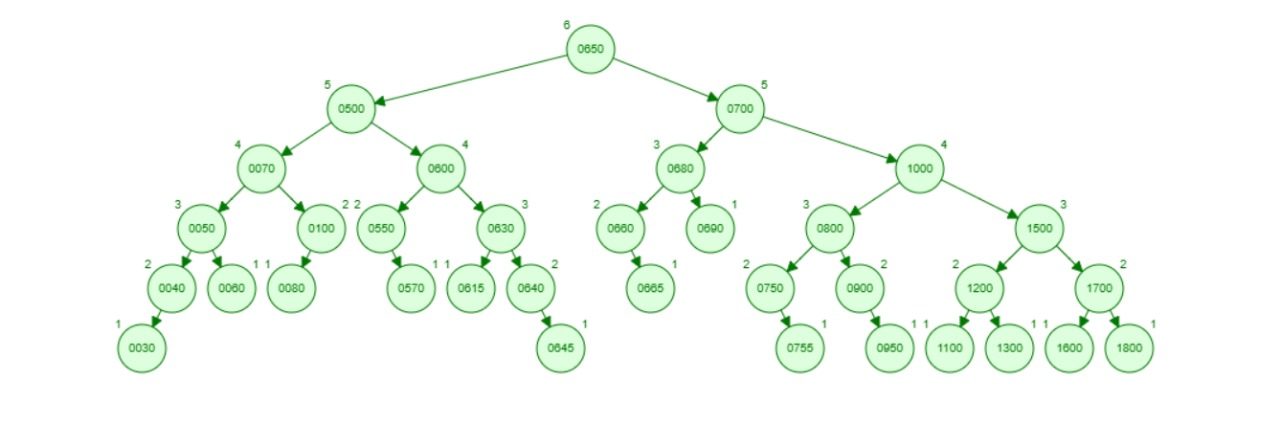
\includegraphics[width=\linewidth]{img/avl_after.jpeg}
         \caption{After inserting node 645}
         \label{fig:af645}
     \end{minipage}
 \end{figure}

 \subsection{Analysis for second dataset}

 The analysis of the second dataset presented significant challenges due to the high volume of data.
 Although it is possible to execute the procedures for all document quantities tested in the first dataset,
 it was observed that the processing time becomes substantially longer.
 Thus, the generation of CSV files and graphs was performed with a sample of 1,000 documents,
 as the execution for the complete set proved to be computationally infeasible, due to the saved statistics and the
 high volume of data.

 \subsubsection{Insertion Performance}

 Table \ref{tab:insercao_db2} presents the performance metrics for insertion operations on the second dataset,
 for different quantities of documents ($n$), analogous to what was done for the first dataset.

 \begin{table}[H]
     \centering
     \begin{tabular}{|c|c|c|c|c|c|}
     \hline
     \textbf{n (docs)} & \textbf{Words} & \textbf{Structure} & \textbf{Time (s)} & \textbf{Comparisons} & \textbf{Relative Efficiency} \\
     \hline
     \multirow{3}{*}{10} & \multirow{3}{*}{7.681} & BST & 0.052 & 542,415 & 1.00 \\
     & & AVL & 0.038 & 546,517 & 0.99 \\
     & & RBT & 0.050 & 502,147 & 1.08 \\
     \hline
     \multirow{3}{*}{100} & \multirow{3}{*}{24.787} & BST & 0.341 & 4,099,770 & 1.00 \\
     & & AVL & 0.320 & 3,969,198 & 1.03 \\
     & & RBT & 0.309 & 3,810,306 & 1.08 \\
     \hline
     \multirow{3}{*}{1000} & \multirow{3}{*}{77.770} & BST & 4.261 & 41,768,444 & 1.00 \\
     & & AVL & 3.433 & 40,481,015 & 1.03 \\
     & & RBT & 4.581 & 39,623,497 & 1.05 \\
     \hline
     \end{tabular}
     \caption{Insertion performance on the second dataset with relative efficiency compared to the BST}
     \label{tab:insercao_db2}
 \end{table}


 In the second dataset, a consistent behavior of the balanced trees is observed in relation to the BST.
 The RBT demonstrates superiority regarding the number of comparisons. The AVL also stands out for its low execution
 time for $n = 1000$.

 Figure \ref{fig:timedist} demonstrates the distribution of insertion time, showing that all trees 
 have very similar variability, differing only in their respective means.

 \begin{figure}[H]
     \centering
     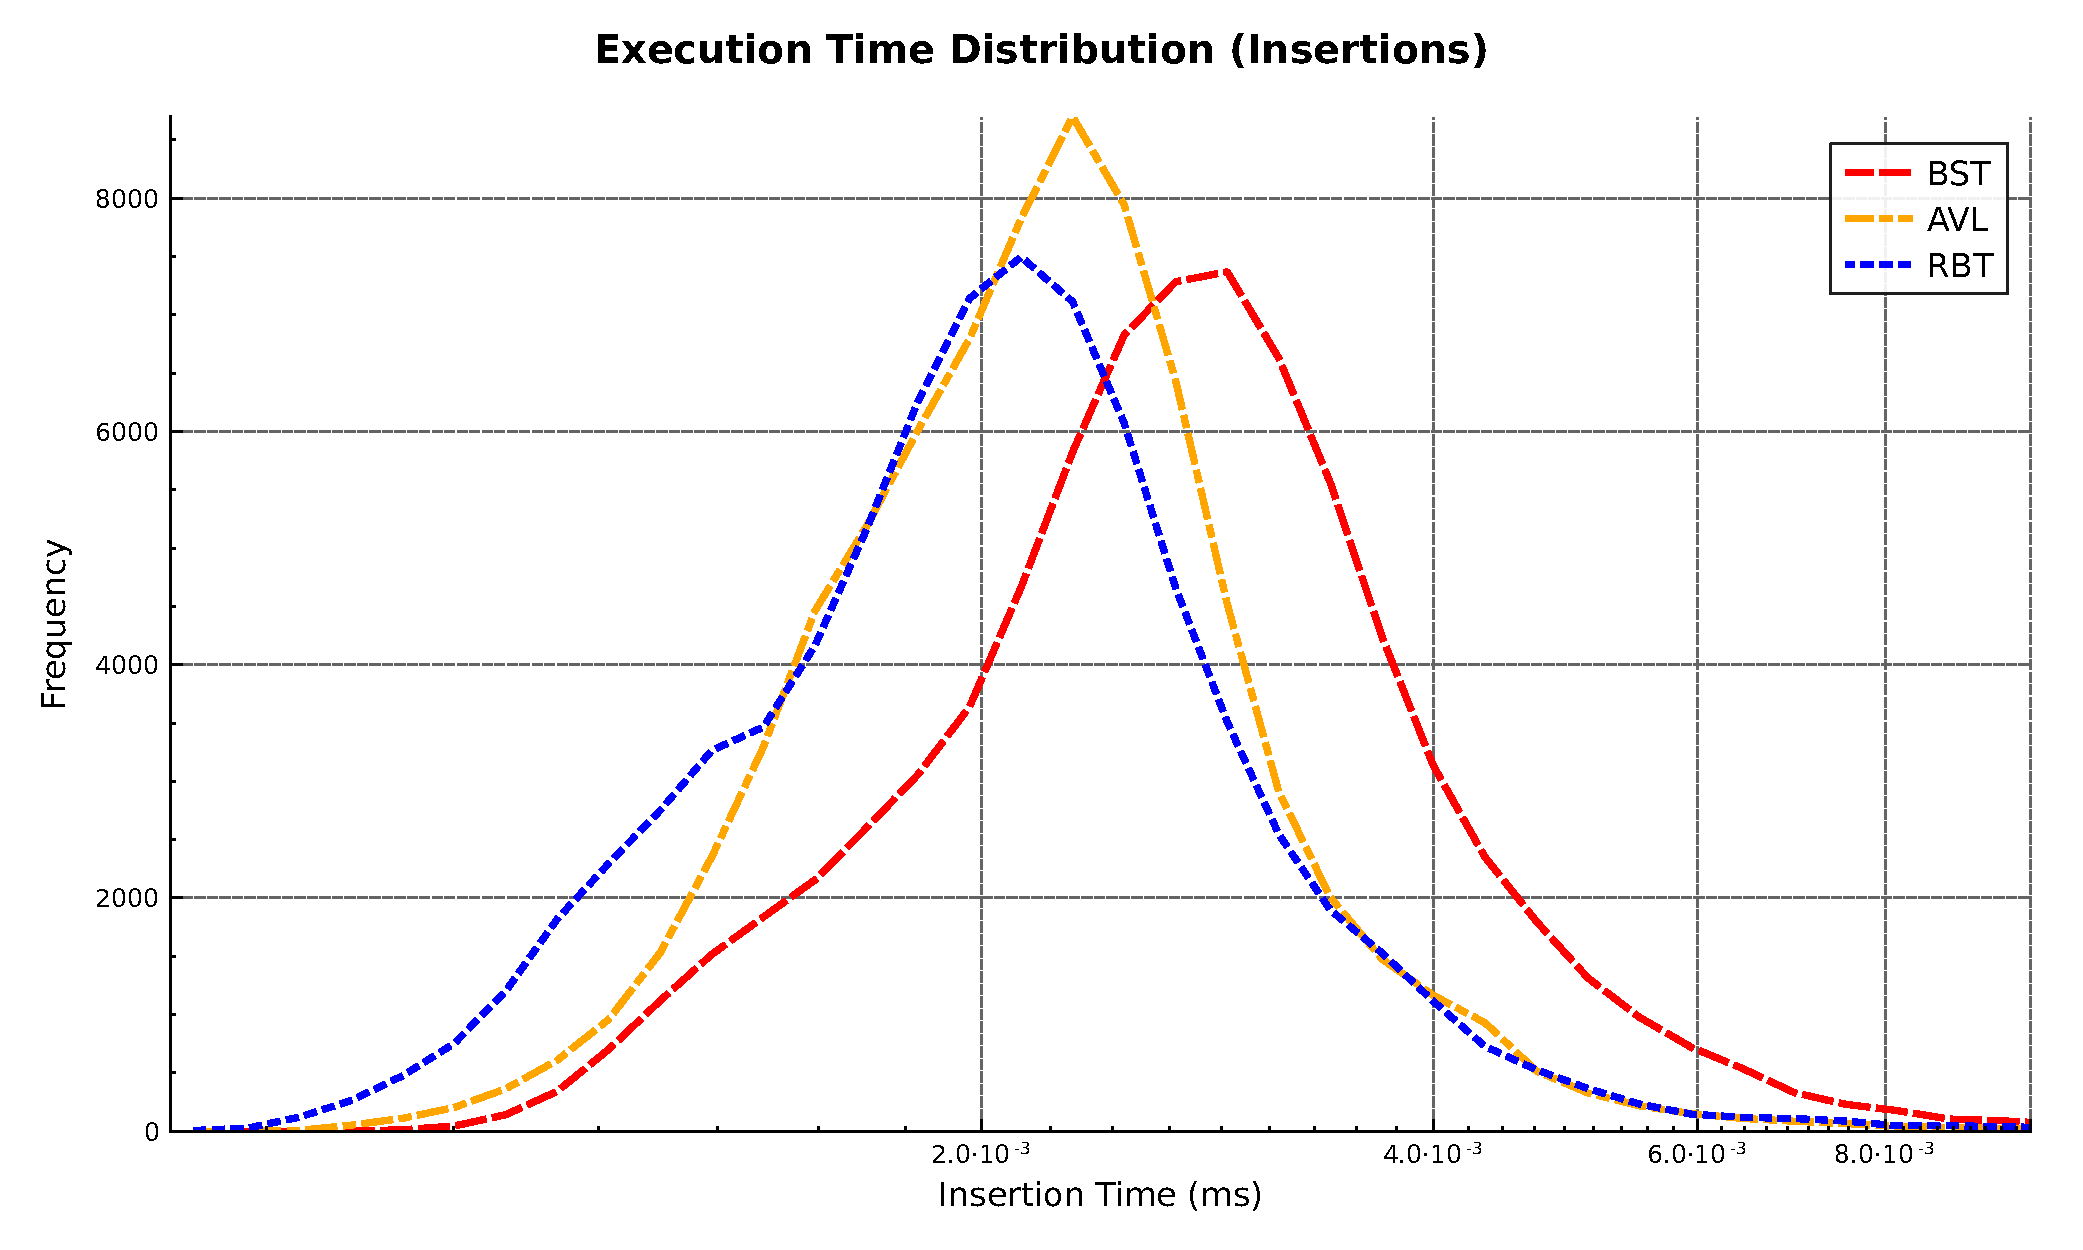
\includegraphics[width=0.8\linewidth]{img/Graph_5_77770.pdf}
     \caption{Number of comparisons by number of words}
     \label{fig:timedist}
 \end{figure}

 Figure \ref{fig:cumulativedist} reveals that, although insertions in AVL and RBT
 involve additional balancing operations, the superior efficiency in search operations
 compensates for this initial cost, particularly in datasets with many repeated words.

 \begin{figure}[H]
     \centering
     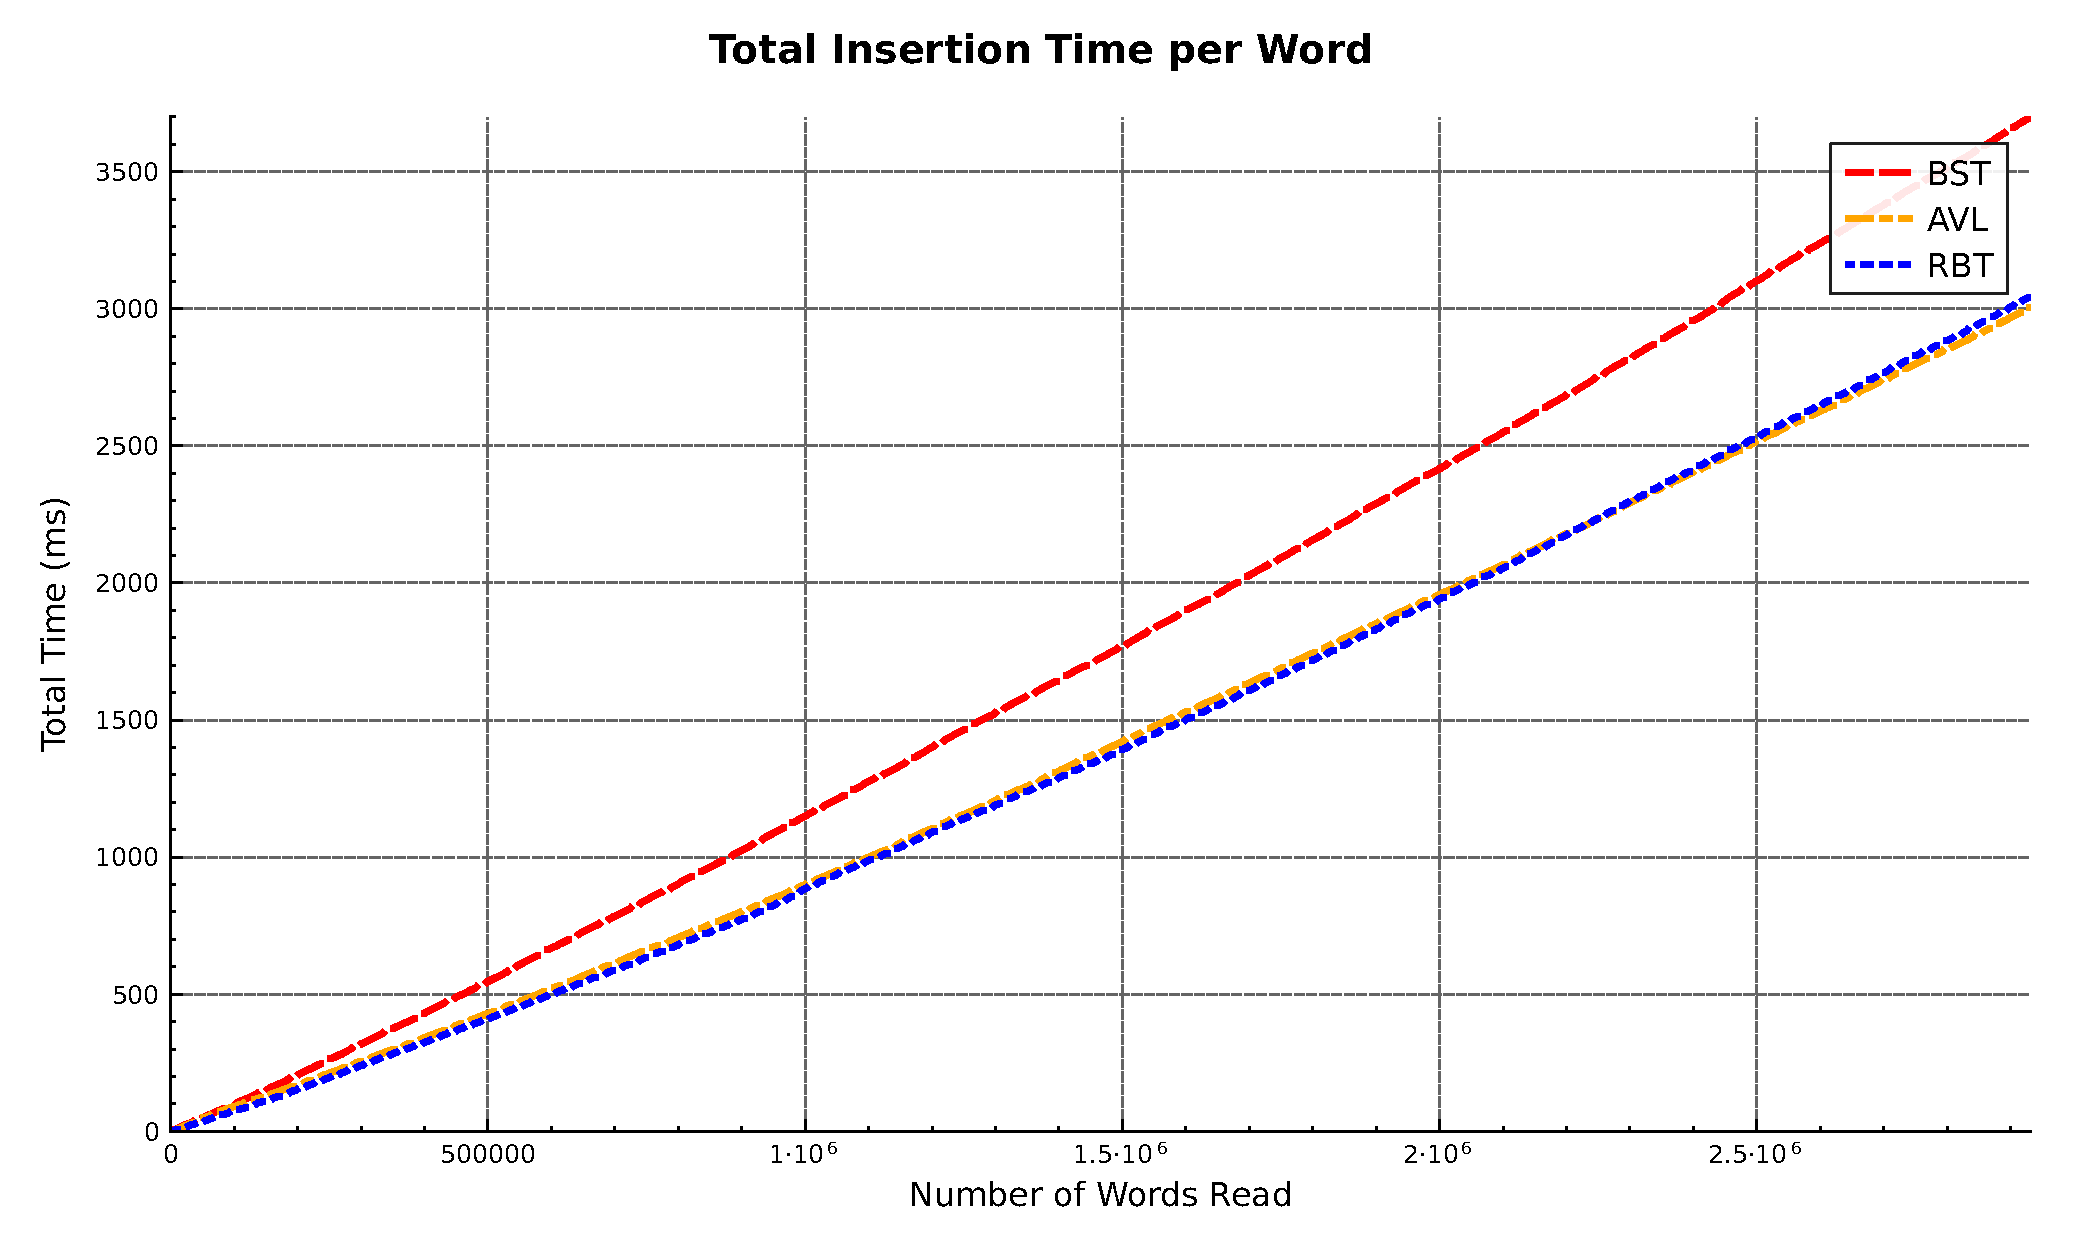
\includegraphics[width=0.8\linewidth]{img/Graph_4_77770.pdf}
     \caption{Number of comparisons by number of words}
     \label{fig:cumulativedist}
 \end{figure}
Figure \ref{fig:mean-log2} shows the average number of comparisons for every 100 new words 
inserted into the trees, similar to the analysis of the first dataset.
\begin{figure}[H]
     \centering
     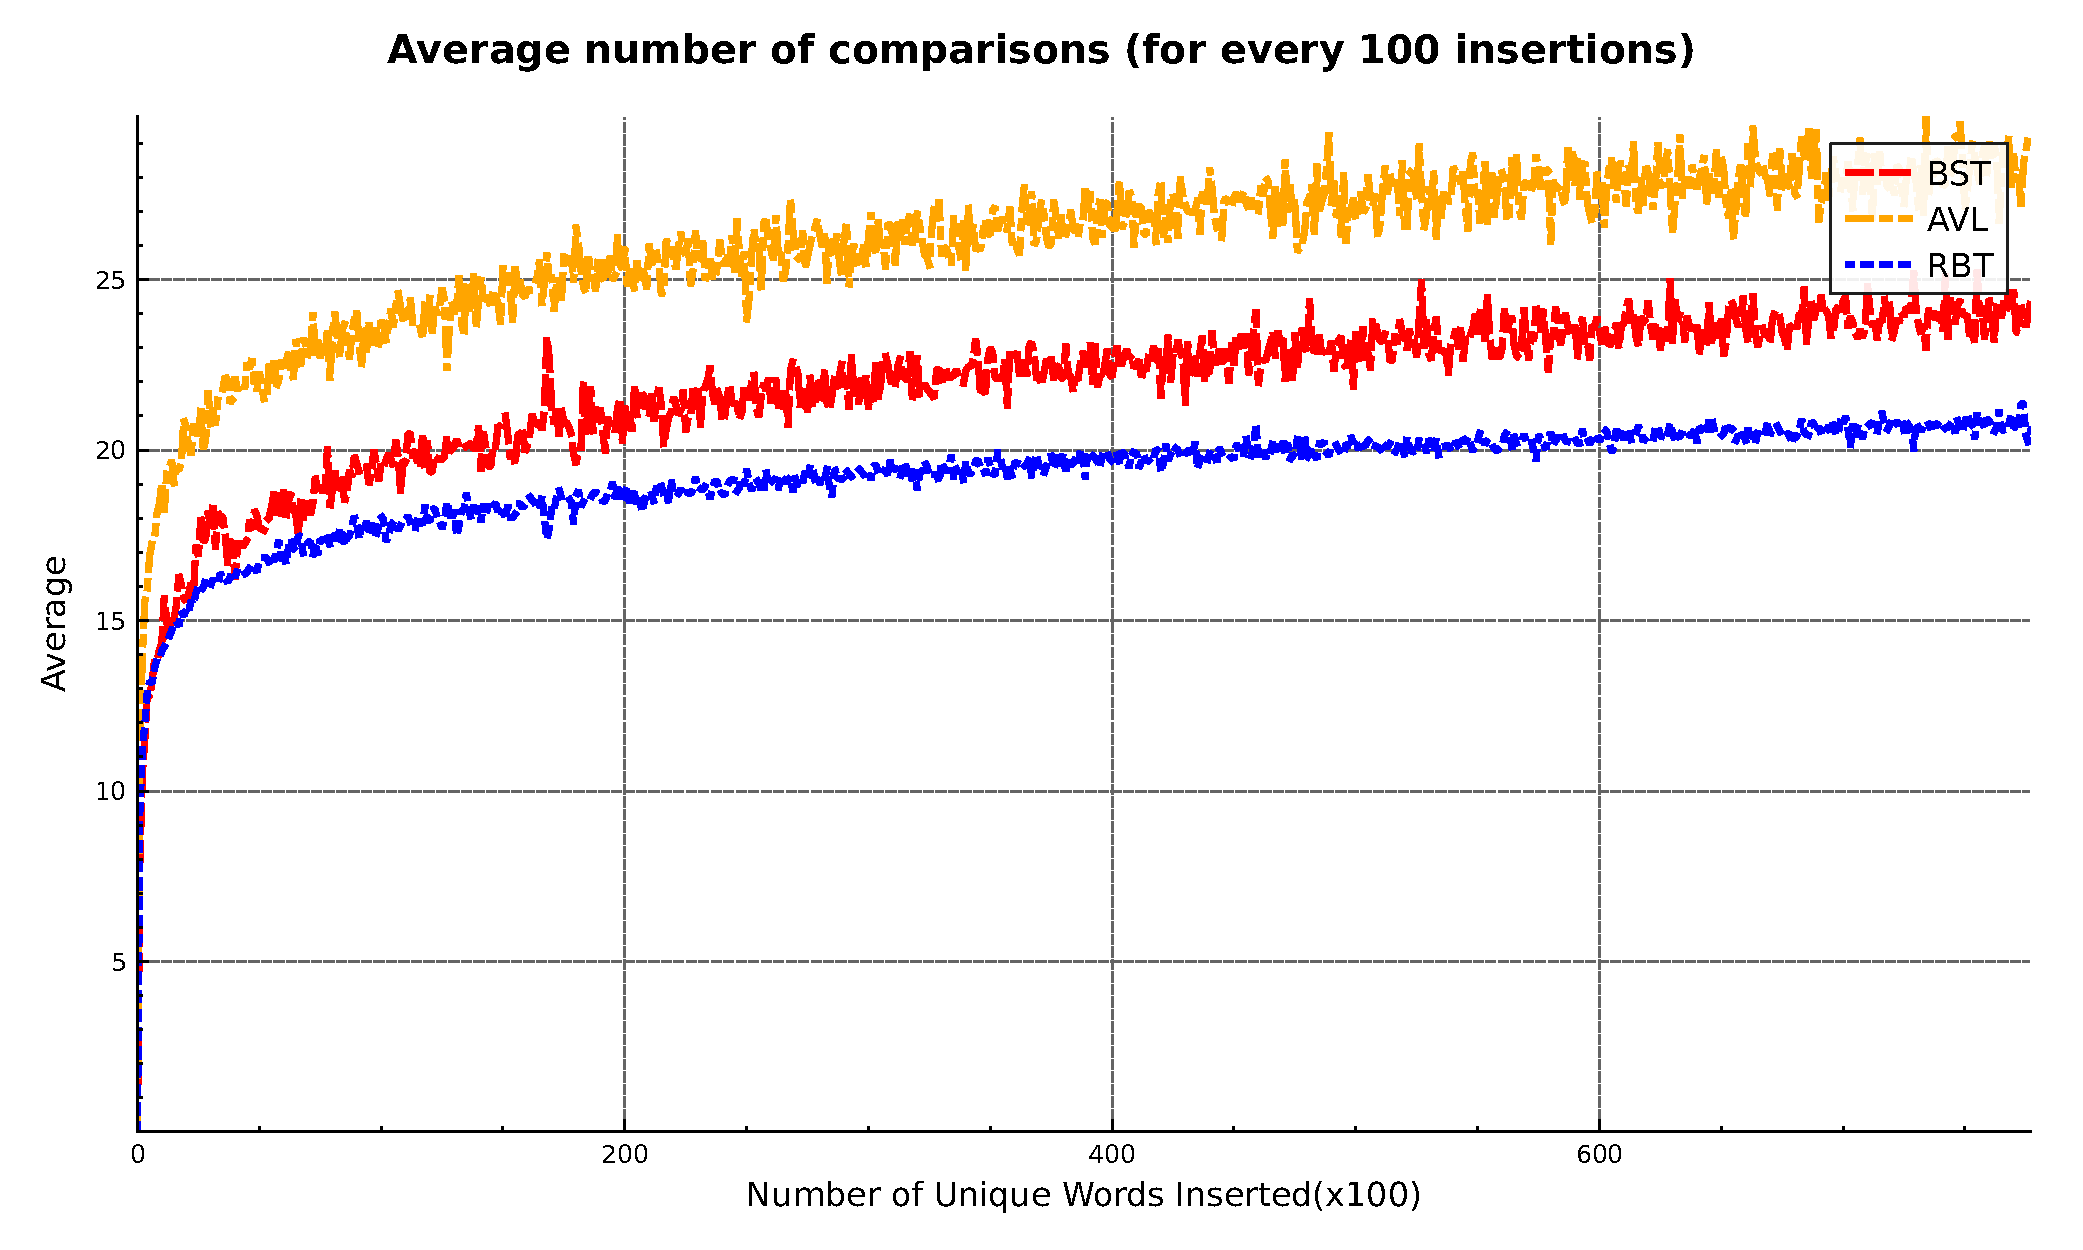
\includegraphics[width=0.8\linewidth]{img/Graph_3_77770.pdf}
     \caption{Number of comparisons by number of words}
     \label{fig:mean-log2}
\end{figure}

As expected, all the graphics is similar to the one from the first dataset.

 \subsubsection{Search Performance}

 Table \ref{tab:busca_db2} displays the results for search operations on the second dataset for different numbers
 of documents ($n$), also analogous to the first dataset.

 \begin{table}[H]
     \centering
     \begin{tabular}{|c|c|c|c|c|c|}
     \hline
     \textbf{n (docs)} & \textbf{Words} & \textbf{Structure} & \textbf{Time (ms)} & \textbf{Comparisons} & \textbf{Relative Efficiency} \\
     \hline
     \multirow{3}{*}{10} & \multirow{3}{*}{7.681} & BST & 3.838 & 121,566 & 1.00 \\
     & & AVL & 4.213 & 93,951 & 1.29 \\
     & & RBT & 4.175 & 94,530 & 1.29 \\
     \hline
     \multirow{3}{*}{100} & \multirow{3}{*}{24.787} & BST & 22.684 & 454,741 & 1.00 \\
     & & AVL & 16.754 & 345,364 & 1.32 \\
     & & RBT & 19.464 & 346,972 & 1.31 \\
     \hline
     \multirow{3}{*}{1000} & \multirow{3}{*}{77.770} & BST & 86.649 & 1,622,044 & 1.00 \\
     & & AVL & 87.532 & 1,213,580 & 1.34 \\
     & & RBT & 80.670 & 1,223,110 & 1.33 \\
     \hline
     \end{tabular}
     \caption{Search performance on the second dataset with relative efficiency compared to the BST}
     \label{tab:busca_db2}
 \end{table}

 The balanced trees demonstrate consistent gains in search operations.
 Both AVL and RBT show better performance than BST regarding the number
 of comparisons. Again, due to having few unique words, the time is somewhat unstable for
 analysis.

Figure \ref{fig:comparacoes2} presents the distribution of the number of comparisons made
 during searches, as a function of the number of words, for the three analyzed structures:
 BST, AVL, and RBT. It is observed that the balanced trees (AVL and RBT) have distributions
 that are significantly more concentrated around a single value, with frequency peaks at
 approximately 13 comparisons—indicating that most words are located after this
 number of steps. In the BST, the distribution is more dispersed, with a peak
 shifted to around 20 comparisons, reflecting greater variability compared to the balanced trees.
 The style of the graph is basically the same as the one from the first dataset.

 \begin{figure}[H]
     \centering
     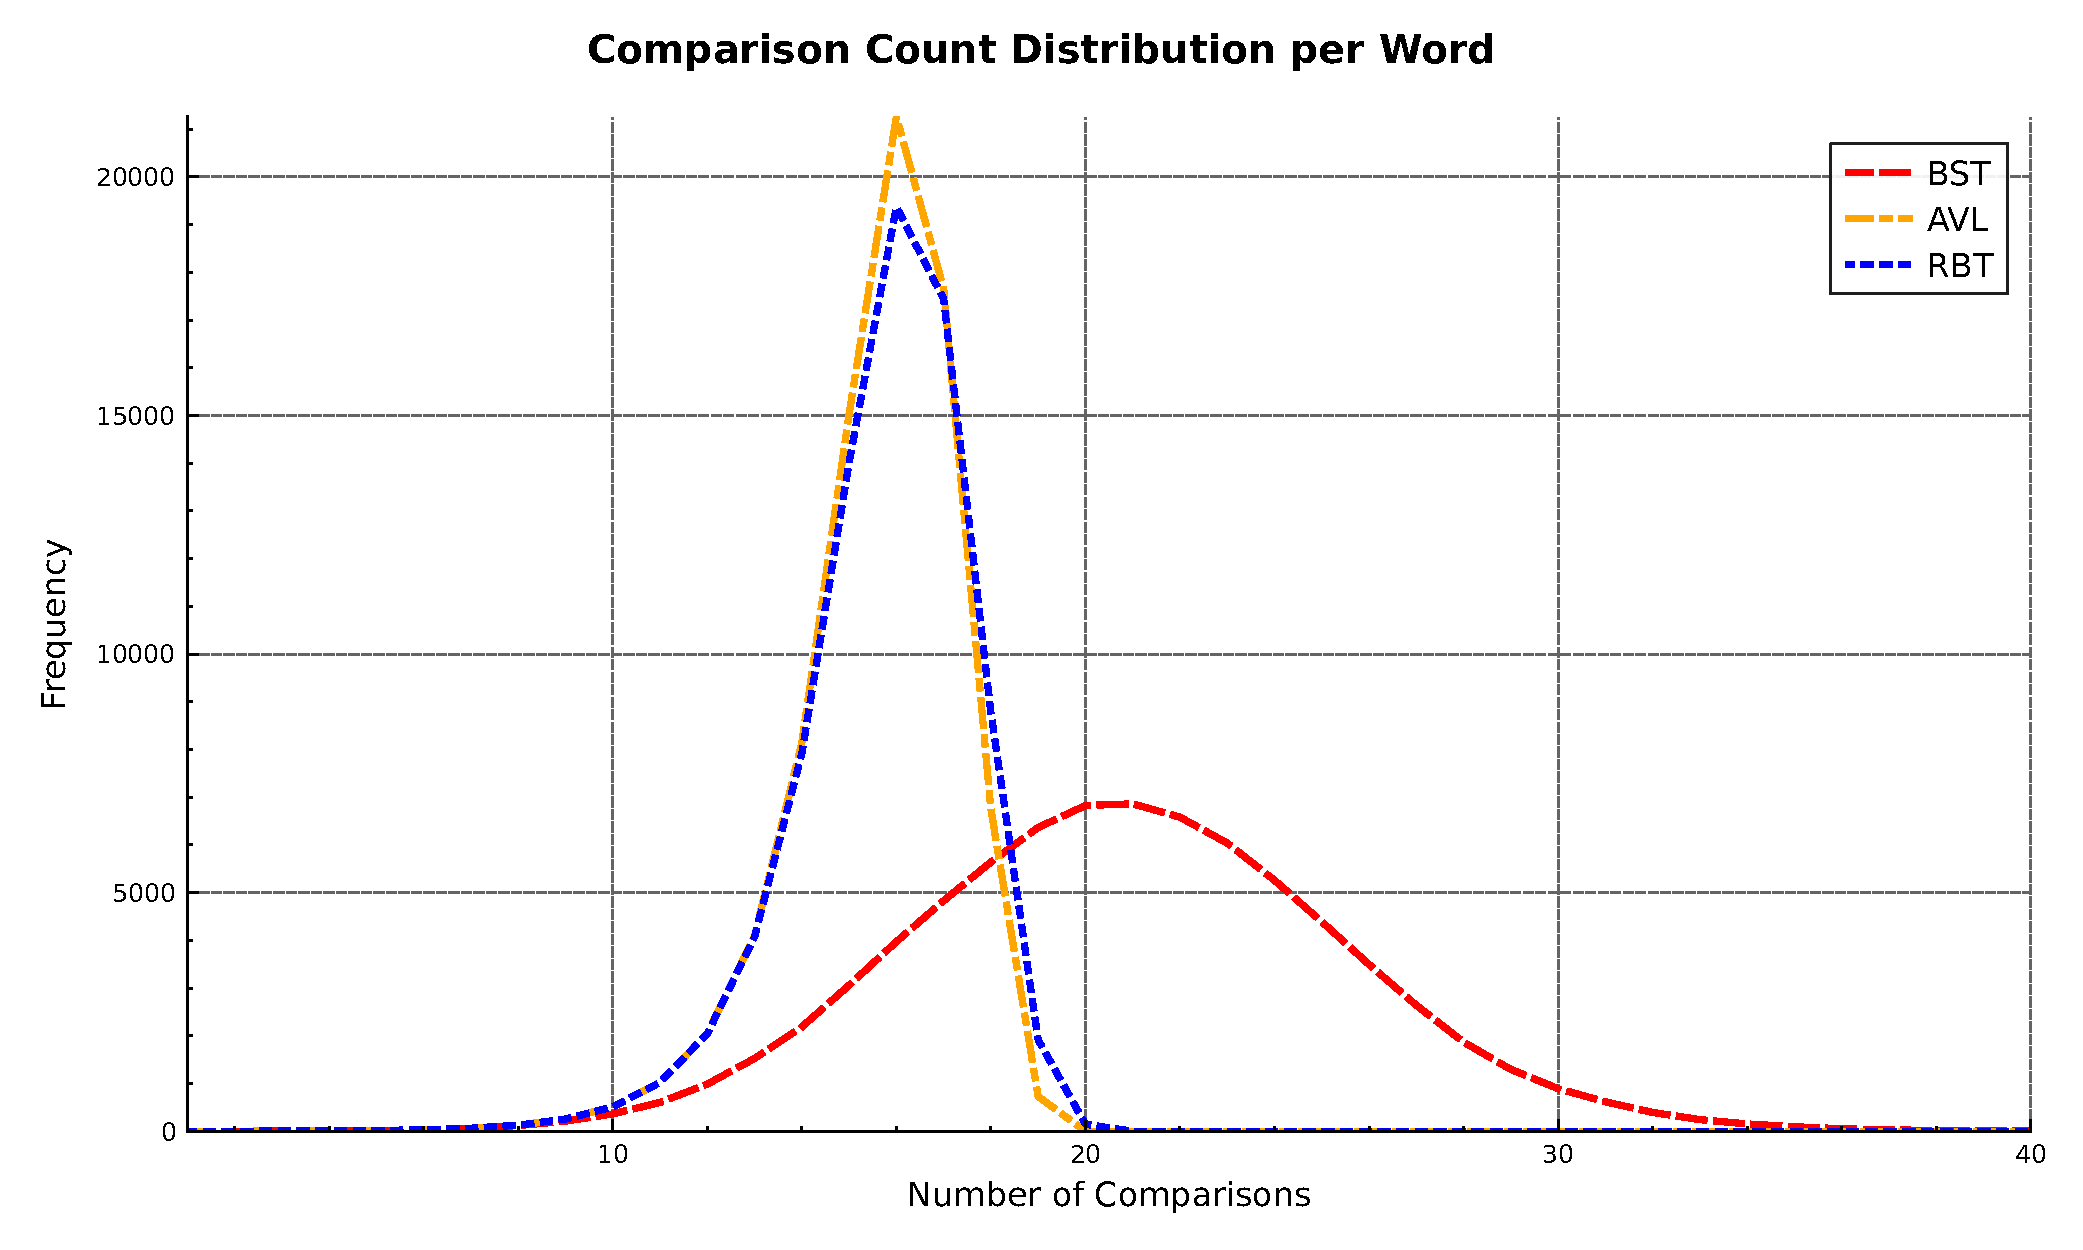
\includegraphics[width=0.8\linewidth]{img/Graph_6_77770.pdf}
     \caption{Number of comparisons by number of words}
     \label{fig:comparacoes2}
 \end{figure}

 \subsubsection{Maximum and Minimum Branch}

 Table \ref{tab:altura_db2} presents the height statistics of the trees in the second dataset,
 with columns analogous to the first data analysis.

 \begin{table}[H]
     \centering
     \begin{tabular}{|c|c|c|c|c|c|c|}
     \hline
     \textbf{n (docs)} & \textbf{Words} & \textbf{Structure} & \textbf{Max. Dist} & \textbf{Min. Dist} & \textbf{Difference} & \textbf{Ratio} \\
     \hline
     \multirow{3}{*}{10} & \multirow{3}{*}{7.681} & BST & 31 & 5 & 26 & 6.20 \\
     & & AVL & 15 & 9 & 6 & 1.67 \\
     & & RBT & 15 & 9 & 6 & 1.67 \\
     \hline
     \multirow{3}{*}{100} & \multirow{3}{*}{24.787} & BST & 34 & 5 & 29 & 6.80 \\
     & & AVL & 17 & 10 & 7 & 1.70 \\
     & & RBT & 17 & 10 & 7 & 1.70 \\
     \hline
     \multirow{3}{*}{1000} & \multirow{3}{*}{77.770} & BST & 40 & 5 & 35 & 8.00 \\
     & & AVL & 18 & 12 & 6 & 1.50 \\
     & & RBT & 19 & 10 & 9 & 1.90 \\
     \hline
     \end{tabular}
     \caption{Tree height statistics for different data volumes in the second dataset}
     \label{tab:altura_db2}
 \end{table}

 The results from the second dataset confirm the patterns observed in the first one even more clearly.
 The BST shows progressive degradation of balancing, with ratios increasing from 6.20 to 8.00.
 In contrast, the balanced structures maintain consistently low ratios: the AVL presents the best ratio for $n=1000$ (1.50),
 while the RBT remains at 1.90. It is noted that the AVL manages to maintain smaller height differences (6 levels for $n=1000$)
 compared to the RBT (9 levels), highlighting its more rigorous balancing. The following graphs
 are on a logarithmic scale for better visualization.

 \begin{figure}[H]
     \centering
     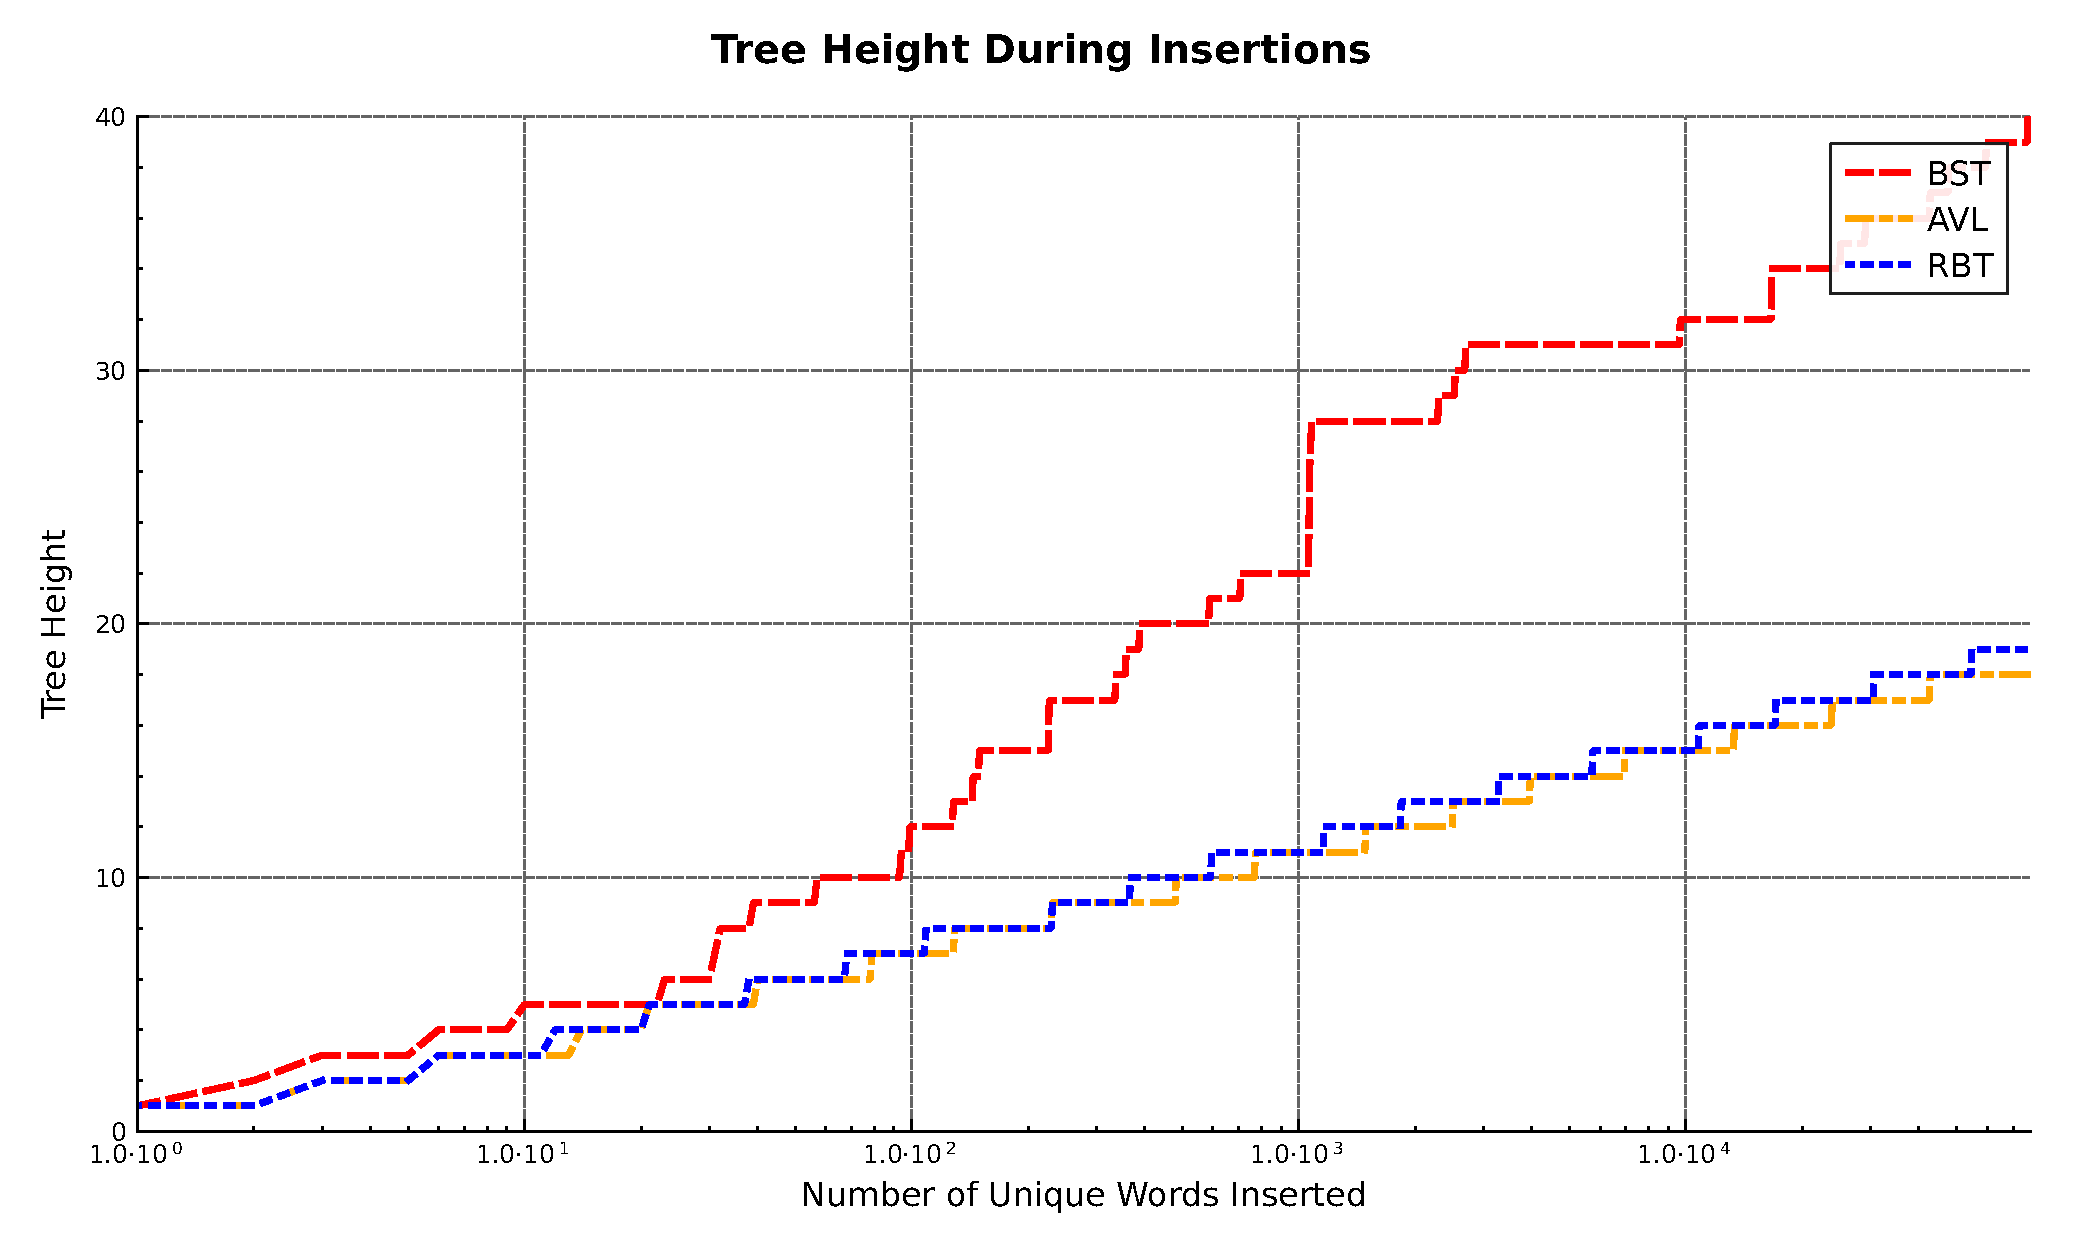
\includegraphics[width=0.75\linewidth]{img/Graph_1_77770.pdf}
     \caption{Tree height per insertion}
     \label{fig:maiorgalho2}
 \end{figure}

 \begin{figure}[H]
     \centering
     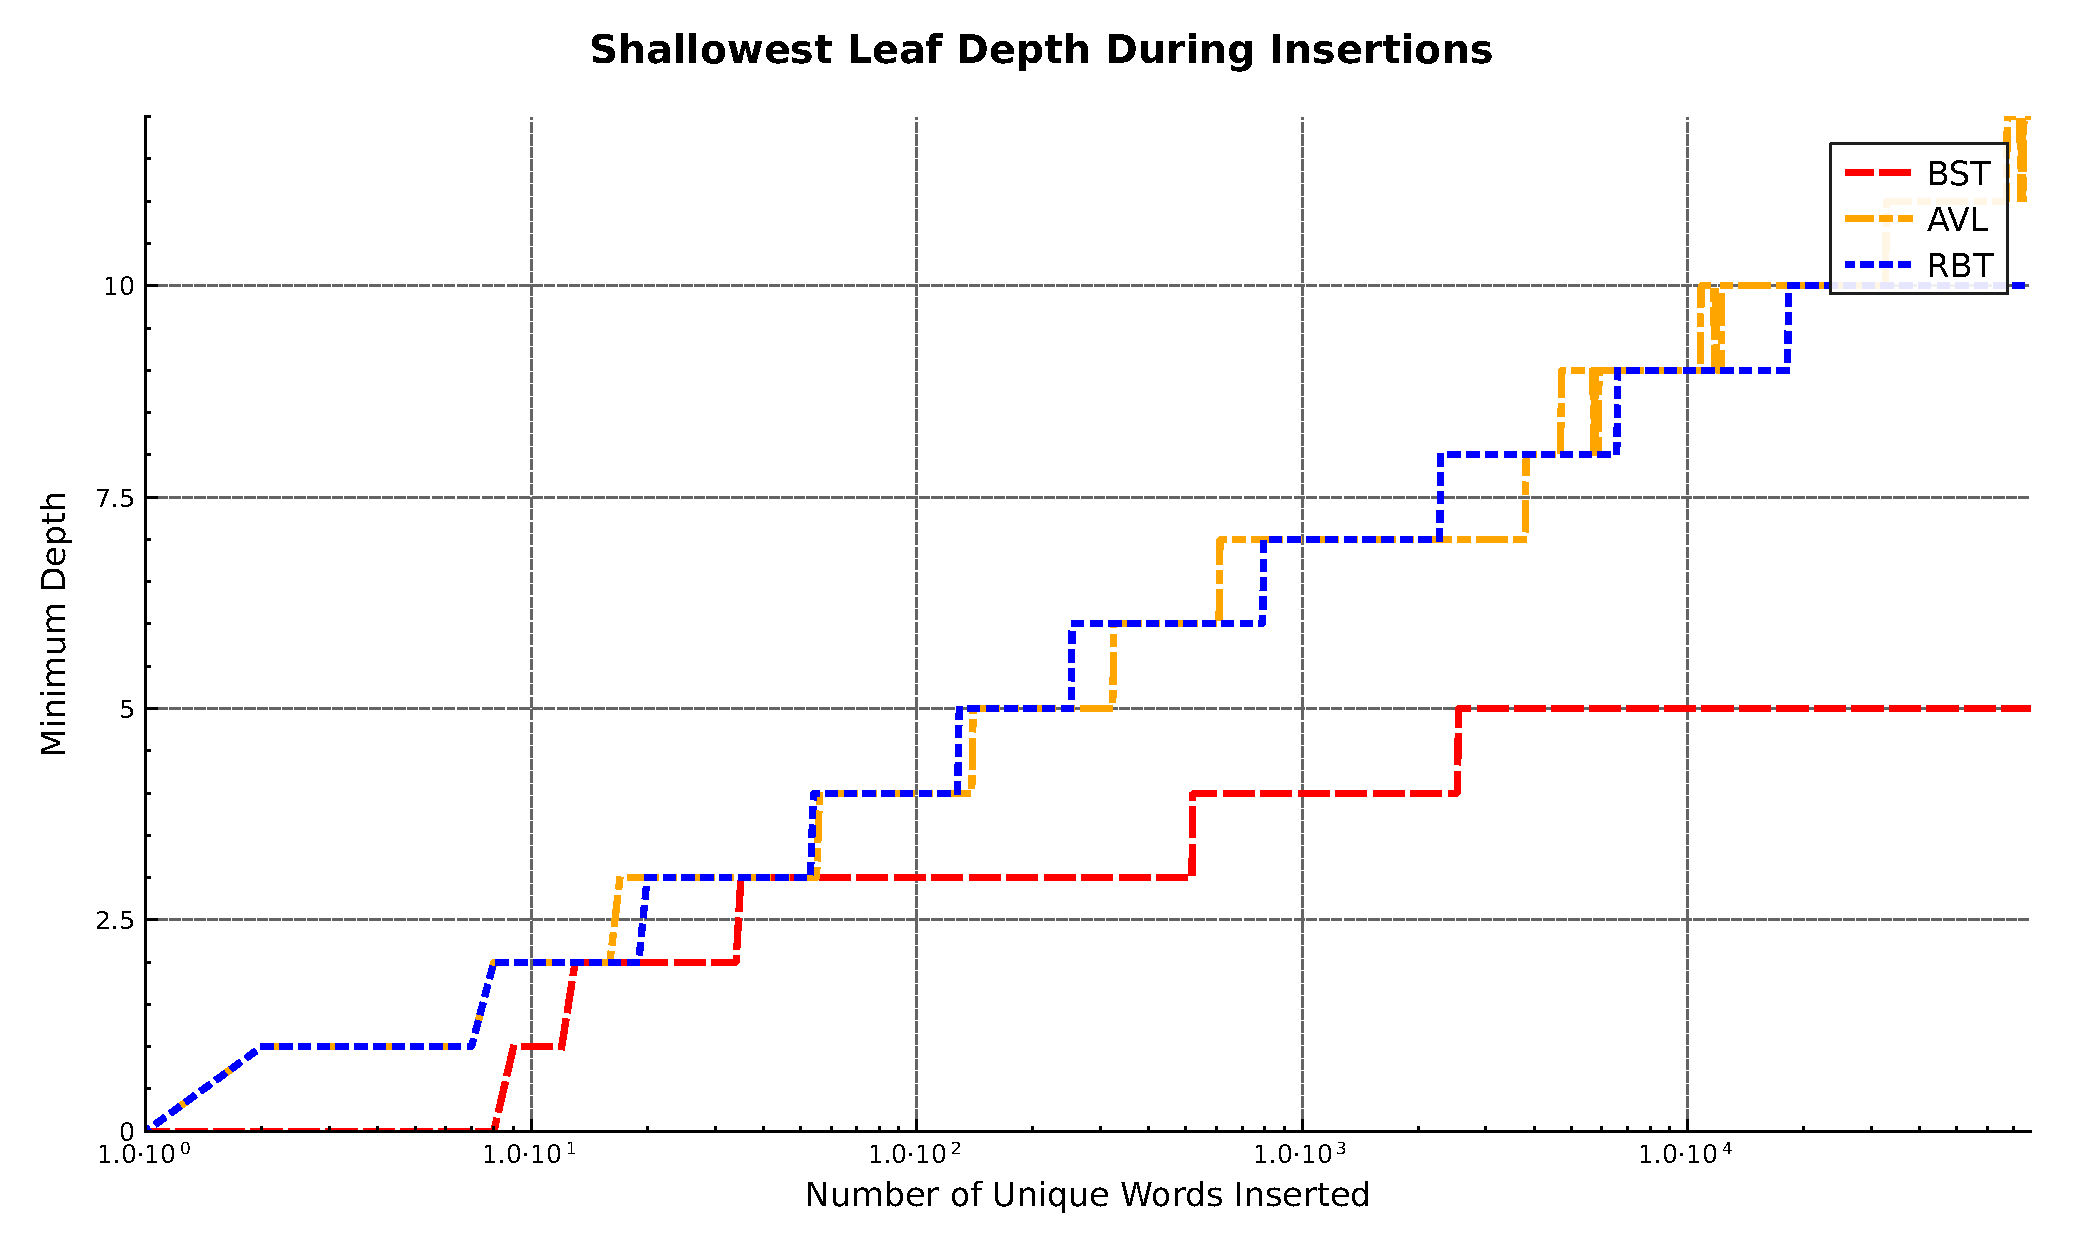
\includegraphics[width=0.75\linewidth]{img/Graph_2_77770.pdf}
     \caption{Tree height per insertion}
     \label{fig:menorgalho2}
 \end{figure}

 Note that, in general, as evidenced by figures \ref{fig:maiorgalho2}-\ref{fig:menorgalho2}, in AVL and RBT trees—being balanced—it is necessary to insert a larger quantity. The analysis is similar to the one 
 for the first dataset.

 \subsection{Conclusion}

 Furthermore, it is observed that the patterns are consistent with those observed in both datasets.
 However, due to the larger number of nodes in this second dataset, the time differences between the approaches
 are more significant, confirming the importance of balanced structures in large-scale applications.

 Comparing the three structures, the BST stands out for its simplicity, but can have poor performance when data is inserted in an orderly fashion—becoming practically a list.
 The AVL tree keeps the tree always very well balanced, which guarantees fast searches, but requires more rotations, making it better for cases with many queries and few insertions.
 The RBT, on the other hand, finds a middle ground: it performs fewer rotations than AVL and still maintains good overall performance, making it a good choice when there are many insertions and modifications to the tree.